\documentclass{article}

% Language setting
\usepackage[spanish]{babel}

% Set page size and margins
\usepackage[a4paper,top=2cm,bottom=2cm,left=3cm,right=3cm,marginparwidth=1.75cm]{geometry}
\usepackage{parskip}

% Useful packages
\usepackage{amsmath}
\usepackage{amssymb}
\usepackage{graphicx}
\usepackage[colorlinks=true, linkcolor=black, urlcolor=blue]{hyperref}

% Uncomment these packages if you want to use dark mode
% \usepackage{darkmode}
% \enabledarkmode

% Title and author
\title{Interpolación de Lagrange}
\author{Álvaro Hernández}
\date{\today}

\begin{document}

%%%%%%%%%%%%%%%%%%%%%%%%%%%%%%%%%%

\maketitle
\tableofcontents
\newpage

\section{Introducción}

En este entregable se hará uso del polinomio interpolador de Lagrange para aproximar una función dada. Se analizarán los distintos métodos para obtener las ventajas y desventajas de cada uno.

Nuestra función dada es:

\begin{equation}\label{funcion}
	5 \cos \left( \frac{\pi x}{3} \right)
\end{equation}

Y los nodos que usaremos serán:

\begin {equation}\label{nodos}
x_{0} = 0 \quad x_{1} = 1 \quad x_{2} = 3
\end{equation}

Por lo que se puede observar que trabajamos con $n = 3$ nodos, y por tanto la dimensión del problema será de 2.

Se formará la función de Lagrange mediante los métdos de Vandermonde, Lagrange y Newton, y en los siguientes apartados se añadirá un nodo más.

\section{Primeros ejercicios}

\subsection{Obtener la cota de error}

Para este primer ejercicio, se formará la cota de error en $x=2$ mediante el teorema del resto cuya fórmula se nos proporciona en los apuntes:

\begin{equation}
	f(x) - T(x) = \frac{f^{(n+1)}(\theta)}{(n+1)!}(x-x_0)^{n+1}
\end{equation}

En este caso tenemos la fórmula para el polinomio de Taylor, pero como el problema de Lagrange es similar, podemos adaptarla para lo que se pide:

\begin{equation}
	f(x) - L(x) = \frac{f^{(n+1)}(\theta)}{(n+1)!}(x - x_0)(x - x_1)\cdots(x - x_n)
\end{equation}

Donde $f^{(n+1)}(\theta)$ será la derivada de orden $n+1$ de f y $\theta$ lo acotaremos según nuestra función.
Volviendo a los valores de (\ref{funcion}) y (\ref{nodos}), como estamos en un problema de dos dimensiones, la derivada será de orden $2+1$.

Por lo tanto, haremos hasta la tercera derivada:

\begin{figure}[h]
	\center
	\includegraphics[width=0.5\textwidth]{src/derivadas.png}
	\caption{Derivadas de hasta orden 3 de nuestra función}
\end{figure}

Una vez teniendo la tercera derivada, se sustituye en la fórmula anterior con los demás valores de los nodos y el punto en donde estamos calculando el error:


\begin{figure}[h]
	\center
	\includegraphics[width=0.5\textwidth]{src/eq2.png}
	\caption{Valores sustituidos en la fórmula}
\end{figure}

\newpage

Se desarrollará la fórmula hasta acotar el seno de nuestra función, el cual teniendo en cuenta los valores entre los que varía, podemos decir que su valor absoluto será menor o igual que 1.

\begin{figure}[h]
	\center
	\includegraphics[width=0.5\textwidth]{src/eq3.png}
	\caption{Desarrollo de la fórmula}
\end{figure}

\begin{figure}[h]
	\center
	\includegraphics[width=0.5\textwidth]{src/eq4.png}
	\caption{Función de error acotada.}
\end{figure}

Por lo que finalmente, el error será:

\begin{equation}\label{funcion}
  \big|f(x) - L(x)\big| < \frac{-5 \pi^3}{81}
\end{equation}


\subsection{Calcular L(x) mediante la matriz de Vandermonde}

Una forma de expresar L(x) es desarrollarlo en base canónica siendo en vez de las derivadas, valores de la función en distintos puntos, en este caso nuestros nodos.

Así, si buscamos los polinomios en la base canónica, usaremos nuestros nodos (\ref{nodos}) para formarlos, de tal forma que:

\begin{equation}
  L(x_{n}) = f(x_{n})
\end{equation}

\begin{equation}
  L(x_{n}) = a_{0} + a_{1}x_{n} + a_{2}x_{n}^{2} + ... + a_{n}x_{n}^{n}
\end{equation}

Si expresamos nuestros polinomios en una única matriz, cuyos coeficientes serán comunes, formaremos la matriz de Vandermonde:


\begin{figure}[ht]
	\center
	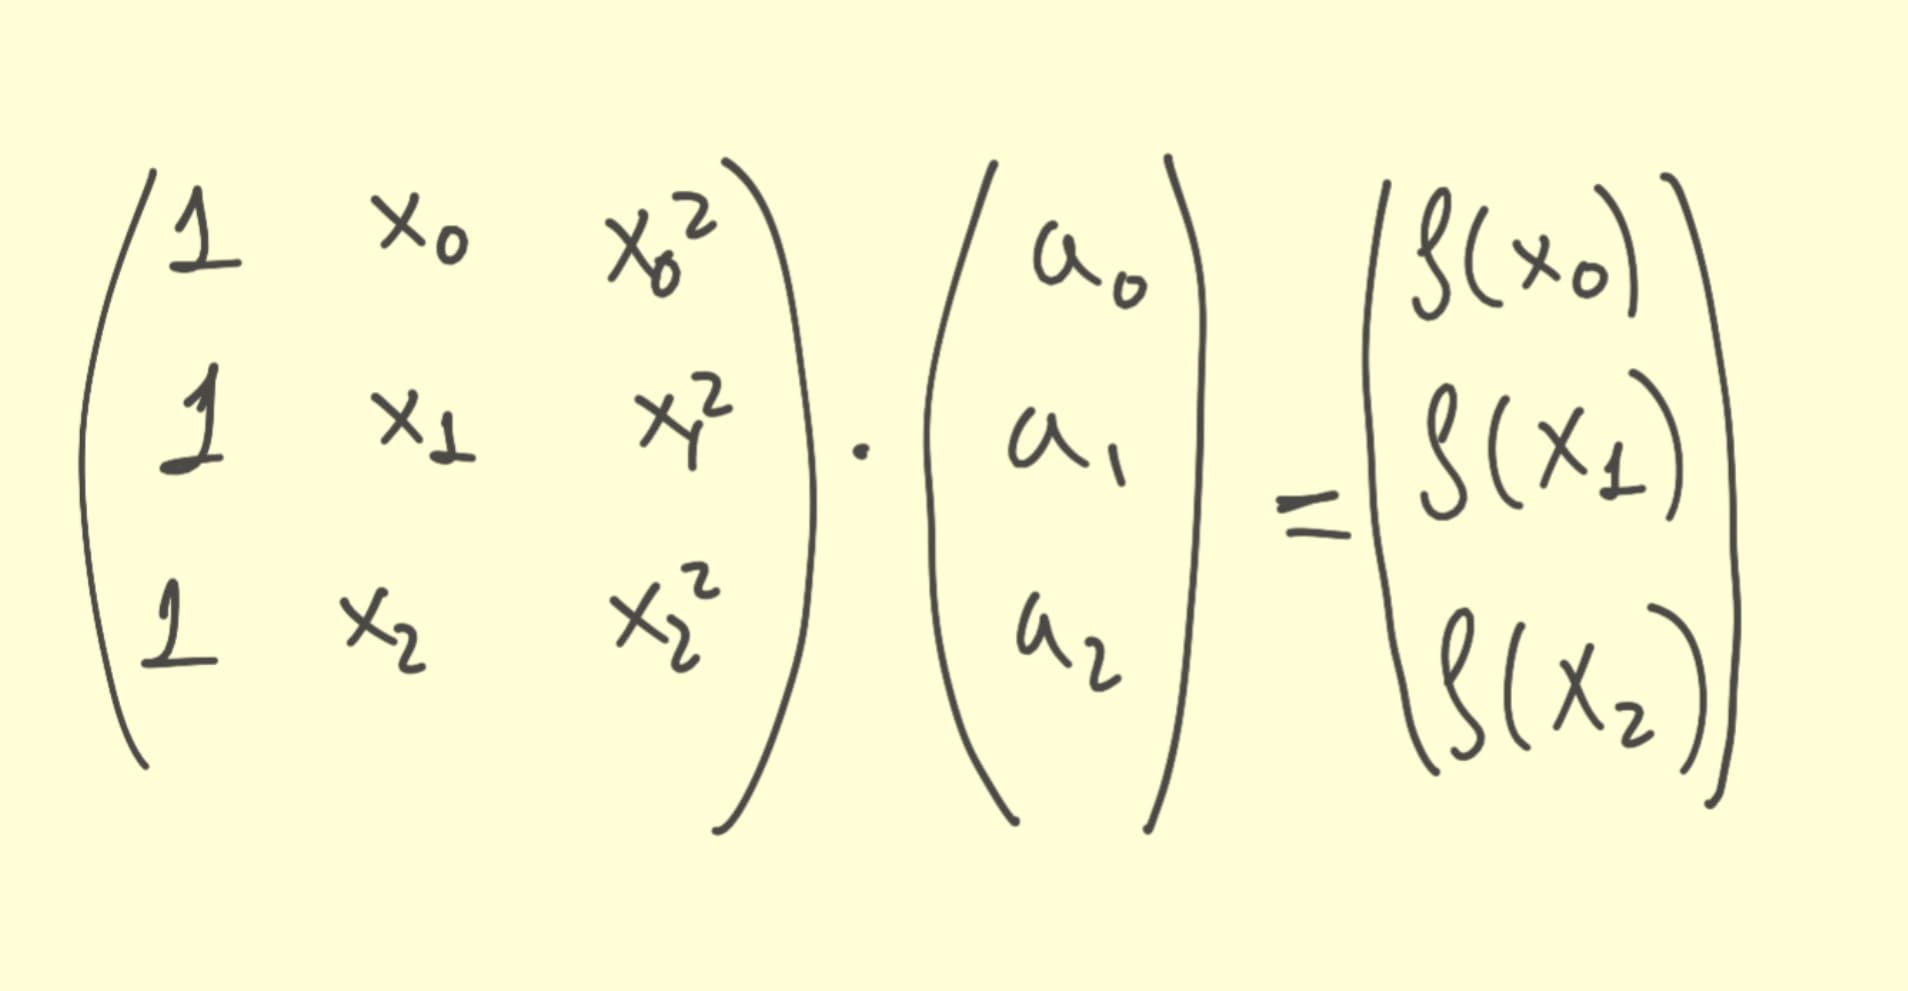
\includegraphics[width=0.5\textwidth]{src/vandermatriz.jpg}
	\caption{Matriz planteada}
\end{figure}

\newpage

Sustituyendo con nuestros nodos y el valor de las funciones:

\begin{figure}[ht]
	\center
	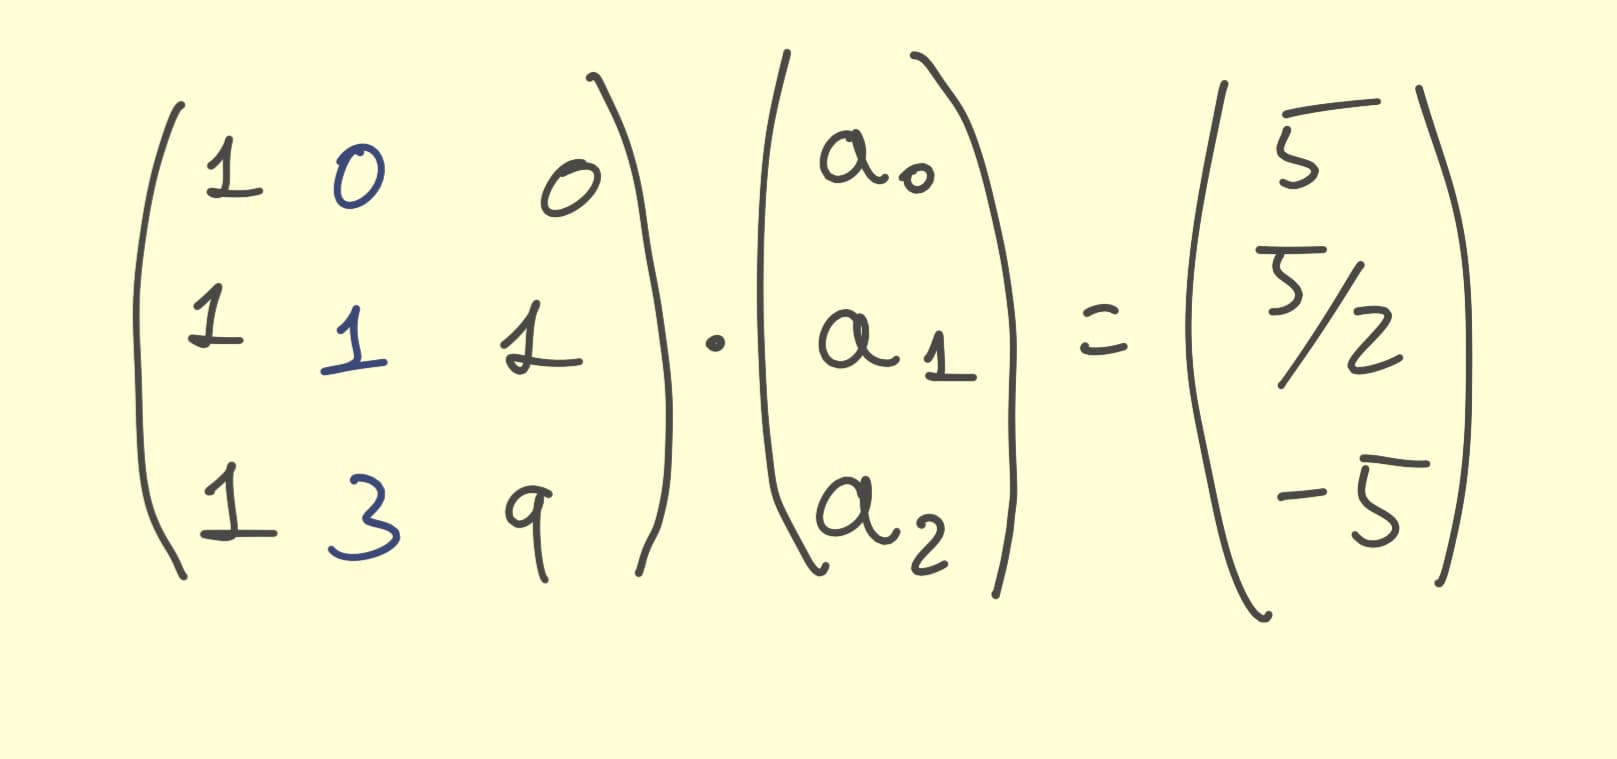
\includegraphics[width=0.5\textwidth]{src/matrizdatos.jpg}
	\caption{Matriz de vandermonde con nuestros datos}
\end{figure}


Si desarrollamos el sistema, podemos determinar inicialmente el valor de $a_{0}$, que será el valor de la función en el primer nodo, y posteriormente desarrollamos el sistema de ecuaciones de segundo grado:

\begin{figure}[ht]
	\center
	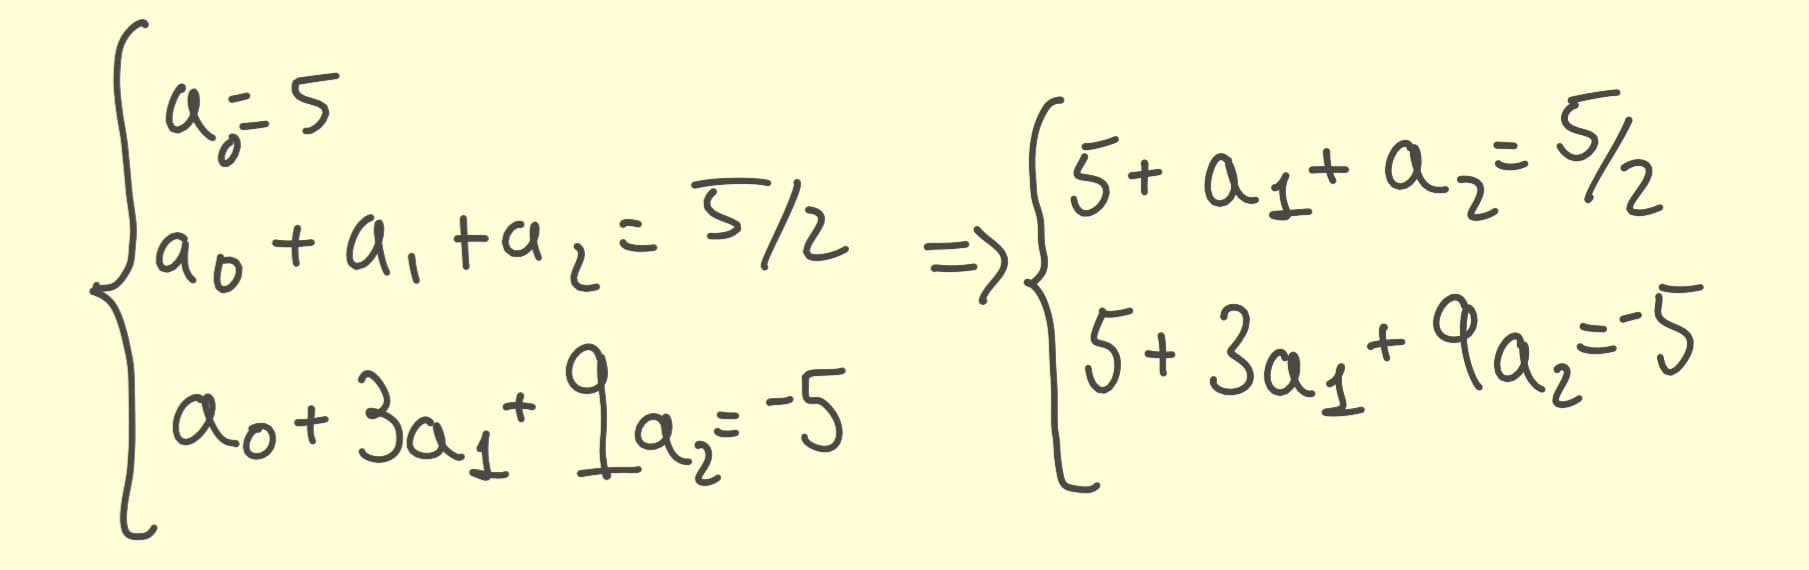
\includegraphics[width=0.5\textwidth]{src/sistemaplanteado.jpg}
	\caption{Planteamiento del sistema}
\end{figure}

Habiendo sacado los coeficientes, tenemos la solución para el problema. Resolvemos mediante Cramer.

\begin{figure}[h]
	\center
	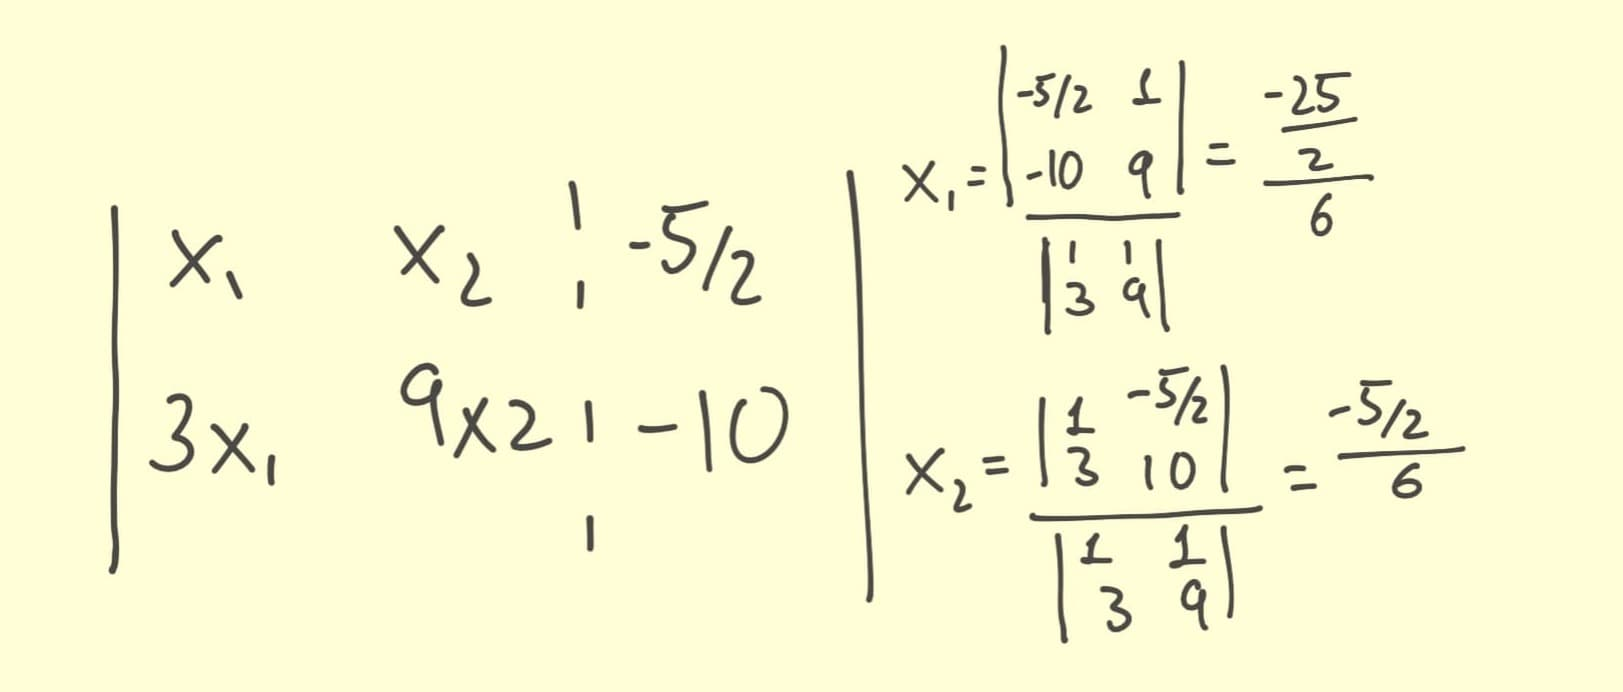
\includegraphics[width=0.5\textwidth]{src/cramer.jpg}
	\caption{Resolución del sistema por cramer}
\end{figure}

Por lo que nuestro polinomio interpolador finalmente será:

\begin{equation}
  L(x) = 5 + -\frac{25}{12}x^{2} + -\frac{5}{12}x
\end{equation}

\newpage


\subsection{Calcular L(x) mediante el método de Lagrange}

En el caso anterior, donde usamos la matriz de Vandermonde, pudimos obtener el polinomio sin mucha dificultad. El problema de la forma anterior, es que para grados n mayores, se hace más complicado de resolver. Por ello, intentamos encontrar una fórmula cerrada para L(x).

Por ello, mediante la forma de Lagrange, tenemos una manera un poco más sencilla de calcular el polinomio interpolador, expresándolo como:

\begin{equation}
  L(x) = \sum_{i=0}^{n} f(x_i) L_i(x) = \sum_{i=0}^{n} f(x_i) \frac{(x - x_0) \dots (x - x_{i-1})(x - x_{i+1}) \dots (x - x_n)}{(x_i - x_0) \dots (x_i - x_{i-1})(x_i - x_{i+1}) \dots (x_i - x_n)}
\end{equation}

De esta forma, expresamos la fórmula sustituyendo con nuestros valores, empezaremos sacando el valor de las funciones en cada nodo:

\begin{figure}[h]
  \center
  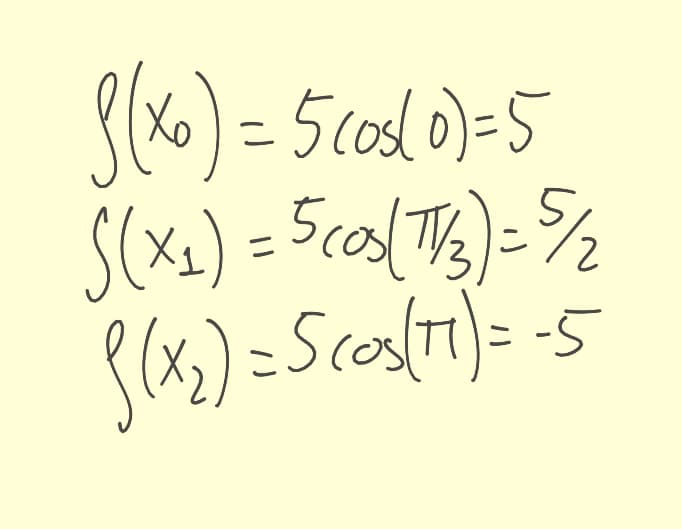
\includegraphics[width=0.3\textwidth]{src/lagrangefis.jpg}
  \caption{Valores de la función en los nodos}
\end{figure} 
  
Ahora, el valor de los polinomios:

\begin{figure}[h]
  \center
  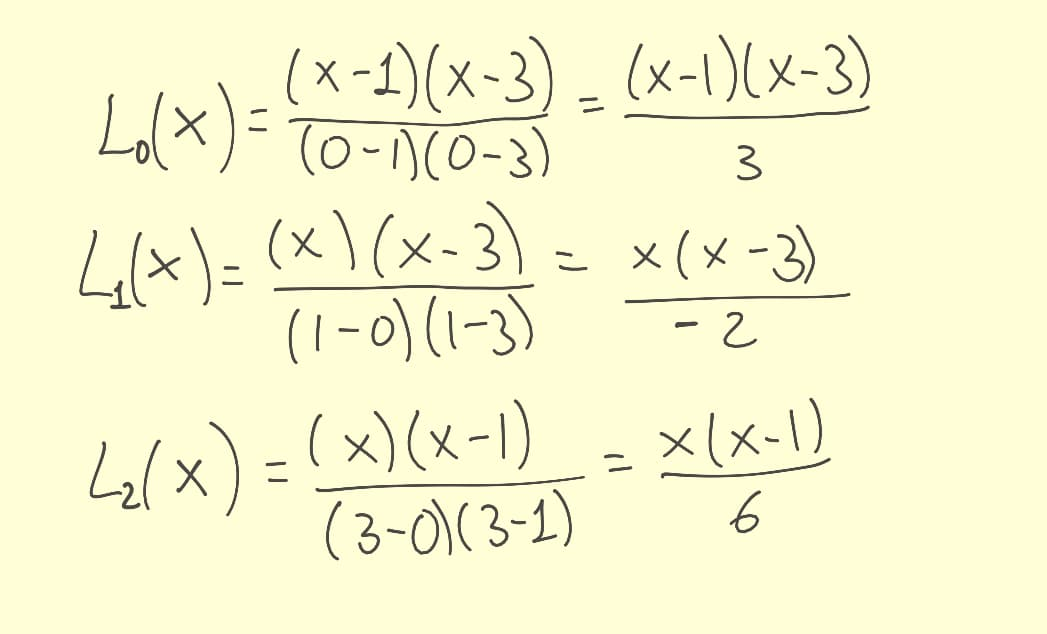
\includegraphics[width=0.5\textwidth]{src/lagrangelis.jpg}
  \caption{Polinomios de Lagrange}
\end{figure}

Por lo que finalmente, si sumamos los correspondientes productos, tendríamos el polinomio interpolador: (hemos hecho la fórmula anterior pero por separado)

\begin{figure}[h]
  \center
  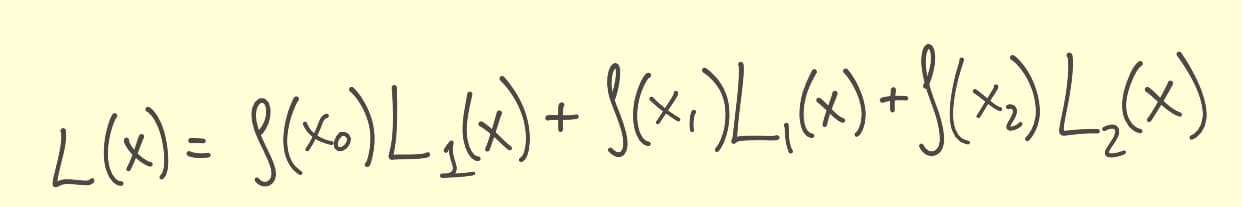
\includegraphics[width=0.5\textwidth]{src/lagrangelx.jpg}
  \caption{Polinomios interpolador sin base canónica}
\end{figure}

Sustituimos con nuestros datos obtenidos:

\begin{equation}
  L(x) = 5 \frac{(x - 1)(x - 3)}{3} + \frac{5}{2} \frac{x(x - 3)}{-2} - 5 \frac{x(x - 1)}{6}
\end{equation}

\subsection{Calcular L(x) mediante la forma de Newton}

Aunque el método de Lagrange nos facilita en parte el problema de situaciones con grados mayores, aún tiene una desventaja, y es el de la "permanencia".

Si quisiéramos añadir un nodo más al problema, de la forma anterior tendríamos que volver a calcular el polinomio sin oportunidad de reusar los cálculos que se hicieron anteriormente. Con la forma de Newton, podemos evitar este inconveniente gracias a la relación de recurrencia que establecimos en clase. En este caso no tenemos una fórmula cerrada, pero sí una forma de calcular el polinomio a partir de los nodos anteriores sin cambiar todo.

Tendremos la expresión del polinomio en la fórmula de Newton con esta base:

\begin{equation}
L(x) = \sum_{i=0}^{n} f[x_0, x_1, \dots, x_{i-1}, x_i](x - x_0)(x - x_1) \dots (x - x_{i-1})
\end{equation}

Y los coeficientes son \textit{diferencias divididas}, que se calculan de la siguiente forma:

\begin{equation}
f[x_0, x_1, \dots, x_{i-1}, x_i] = \frac{f[x_1, \dots, x_{i-1}, x_i] - f[x_0, x_1, \dots, x_{i-1}]}{x_i - x_0} \quad \text{si } i > 0 
\end{equation}

Podemos observar mediante el esquema hecho en clase, que los coeficientes que usaremos serán $f[x_0]$, $f[x_0,x_1]$, y $f[x_0, x_1, x_2]$, pero para ello tendremos que sacar los anteriores también. Es decir, para el $f[x_0, x_1]$ necesitaremos las diferencias calculadas en $x_0$ y $x_1$.

\begin{figure}[h]
  \center
  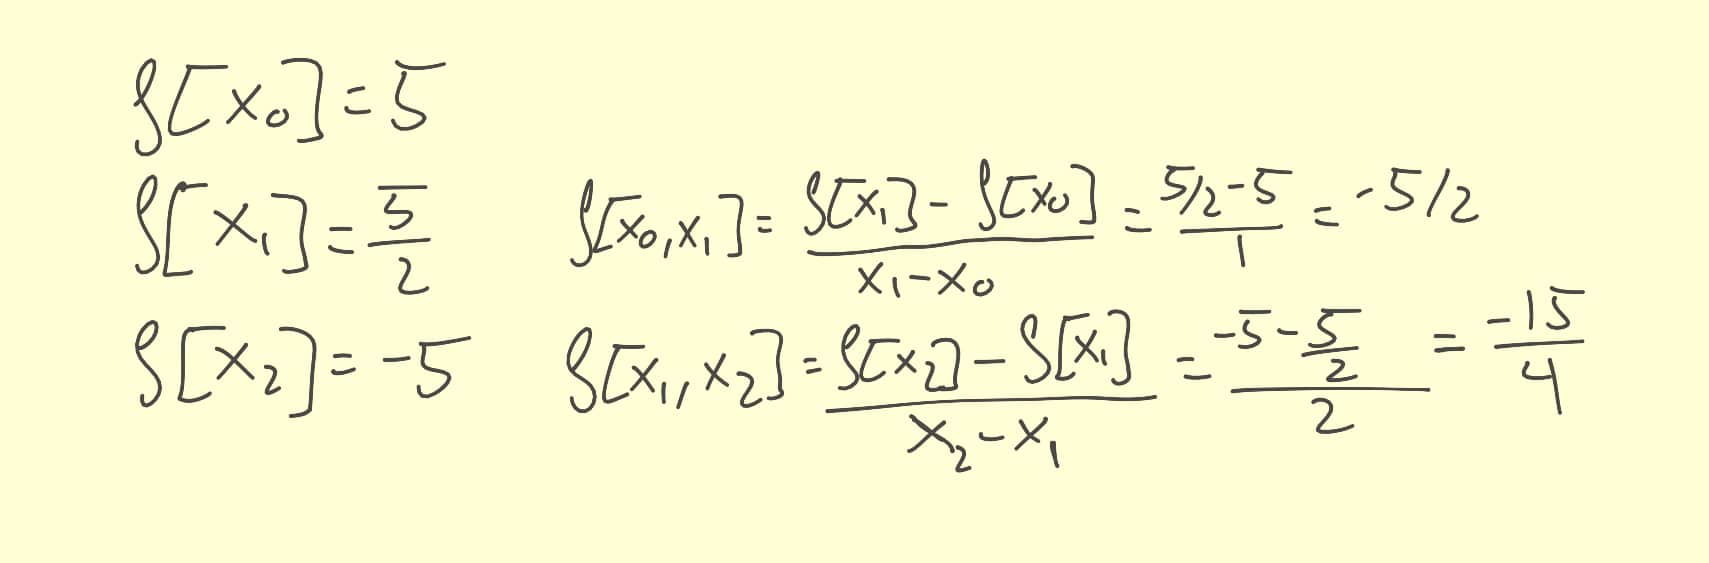
\includegraphics[width=0.7\textwidth]{src/fxnewton.jpg}
  \caption{Diferencias divididas}
\end{figure}

Y finalmente:

\begin{figure}[h]
  \center
  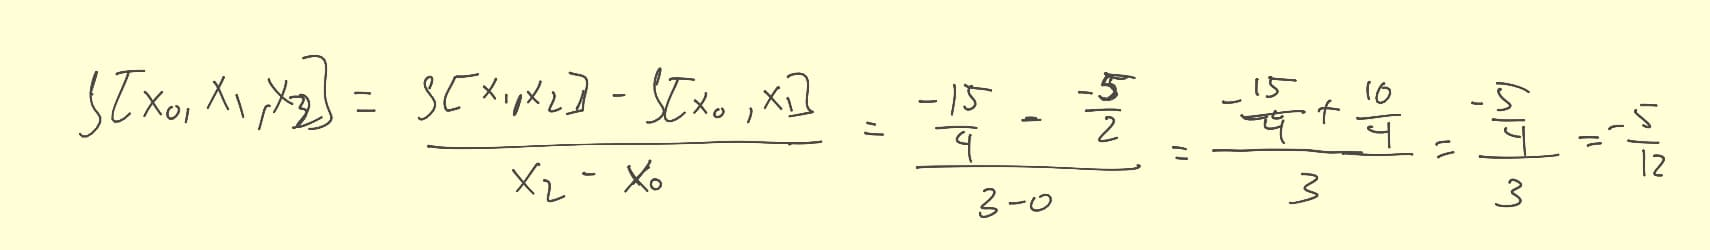
\includegraphics[width=0.7\textwidth]{src/f012newton.jpg}
  \caption{Última diferencia dividida}
\end{figure}

Por lo que como tenemos que multiplicar las diferencias mencionadas anteriormente por la base, quedaría finalemnte:

\begin{figure}[h]
  \center
  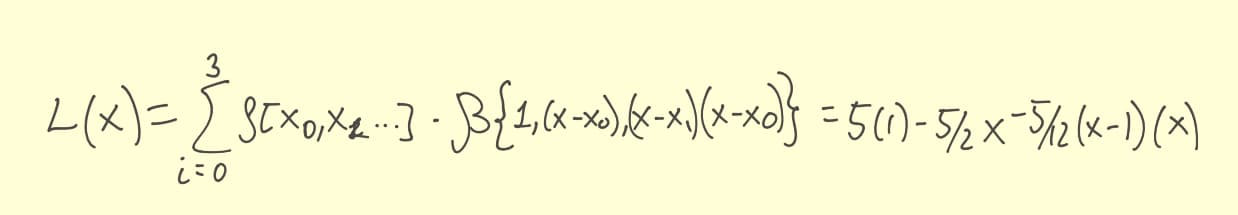
\includegraphics[width=0.7\textwidth]{src/newtonsol1.jpg}
  \caption{Diferencias divididas}
\end{figure}

\newpage


\subsection{Reescribir}

Para esta sección, reescribiremos el polinomio de Lagrange obtenido con los métodos de Lagrange y de Newton, ya que no están en la forma canónica.

Con el método de Lagrange, vamos multiplicando todo e intentando simplificar y finalmente tenemos:

\begin{figure}[h]
  \center
  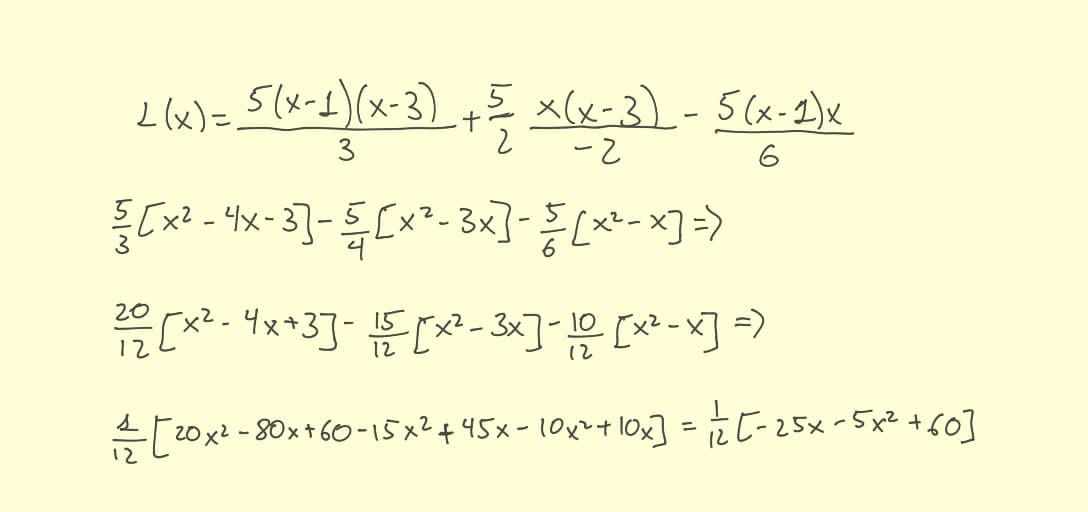
\includegraphics[width=0.7\textwidth]{src/expresionbase1.jpg}
  \caption{Lagrange en base canónica}
\end{figure}

y finalmente, multiplicando esa fracción final, nos queda la base canónica:

\begin{equation}
  L(x) = 5 + -\frac{25}{12}x^{2} + -\frac{5}{12}x
\end{equation}

Para la parte de Newton, usamos la expresión obtenida de la figura 14 y si seguimos operando finalmente nos queda:

\begin{figure}[h]
  \center
  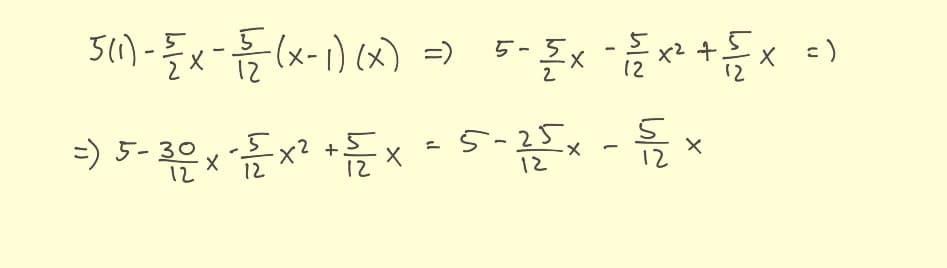
\includegraphics[width=0.7\textwidth]{src/expresionbase2.jpg}
  \caption{Lagrange en base canónica}
\end{figure}

\newpage

\section{Segundos ejercicios}

En estos segundos ejercicios, como ya tenemos la teoría explicada, se hará un desarrollo similar, pero con un nodo más. En este caso, se añadirá el nodo $x_{3} = 6$.

Compararemos finalmente la diferencia para recalcular las soluciones con las distintas formas.

\subsection{Recalcula el nuevo L(x) mediante Vandermonde}

Seguiremos los mismos pasos que cuando atneriormente calculamos la matriz de Vandermonde, solo que ahora tendrá un nodo más:

\begin{figure}[h]
  \center
  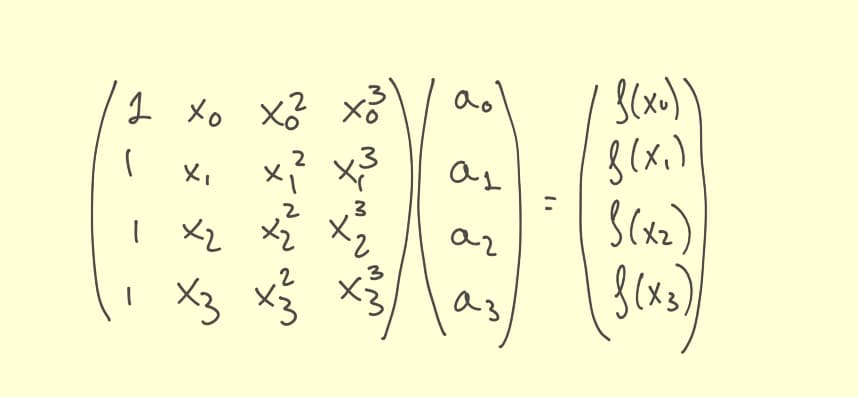
\includegraphics[width=0.7\textwidth]{src/vandermonde2_1.jpg}
  \caption{Lagrange en base canónica}
\end{figure}

Susitituimos por nuestros valores y formamos la ecuación a resolver, como antes, la solución $a_{0}$ es el valor del primer nodo, 5. 

\begin{figure}[h]
  \center
  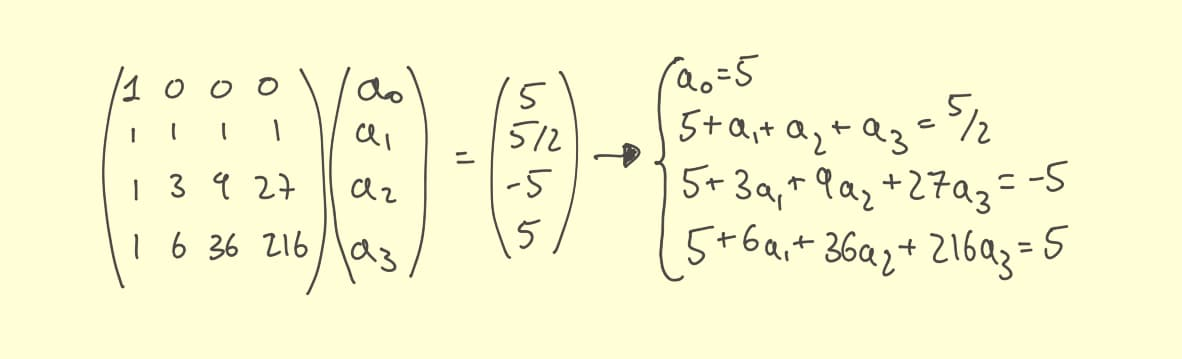
\includegraphics[width=0.7\textwidth]{src/vandermonde2_2.jpg}
  \caption{Lagrange en base canónica}
\end{figure}

Con los 5 de la izquierda ya despejados, formamos ahora la matriz para resolver el sistema de ecuaciones, como antes, usando Cramer. Resolvemos el determinante ya que nos hará falta después: 

\begin{figure}[h]
  \center
  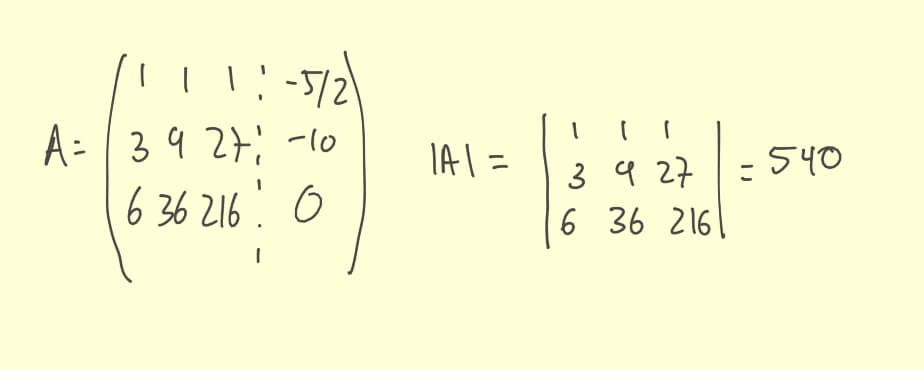
\includegraphics[width=0.7\textwidth]{src/vandermonde2_3.jpg}
  \caption{Lagrange en base canónica}
\end{figure}

Ahora ya podemos sustituir la fila de los valores según queramos calcular $a_1$, $a_2$, o $a_3$. Terminamos de resolver el sistema:

\begin{figure}[h]
  \center
  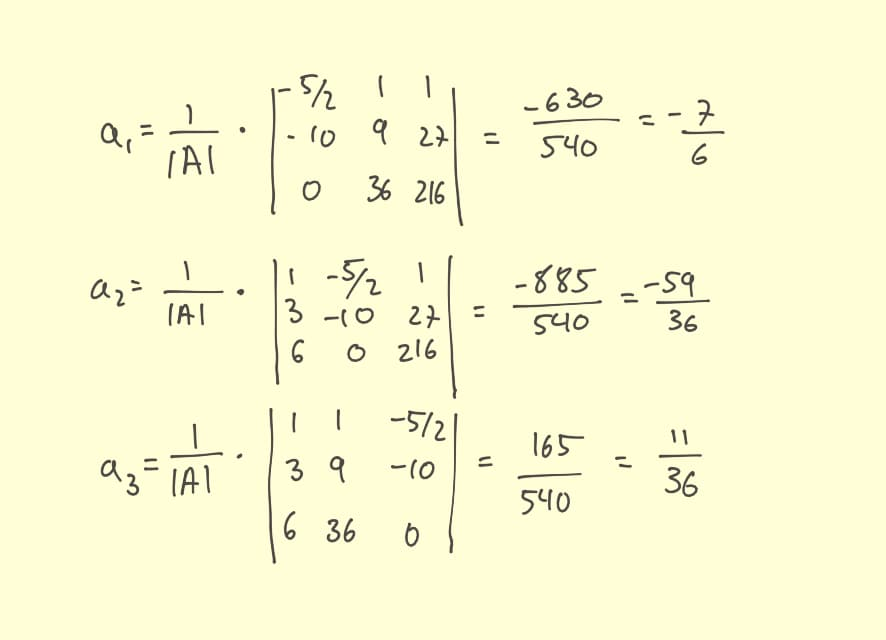
\includegraphics[width=0.7\textwidth]{src/vandermonde2_4.jpg}
  \caption{Lagrange en base canónica}
\end{figure}

Una vez teniendo los valores, como se ha visto en la ecuacion 7, podemos usarlos para formar el polinomio interpolador en la forma canónica:




\end{document}

